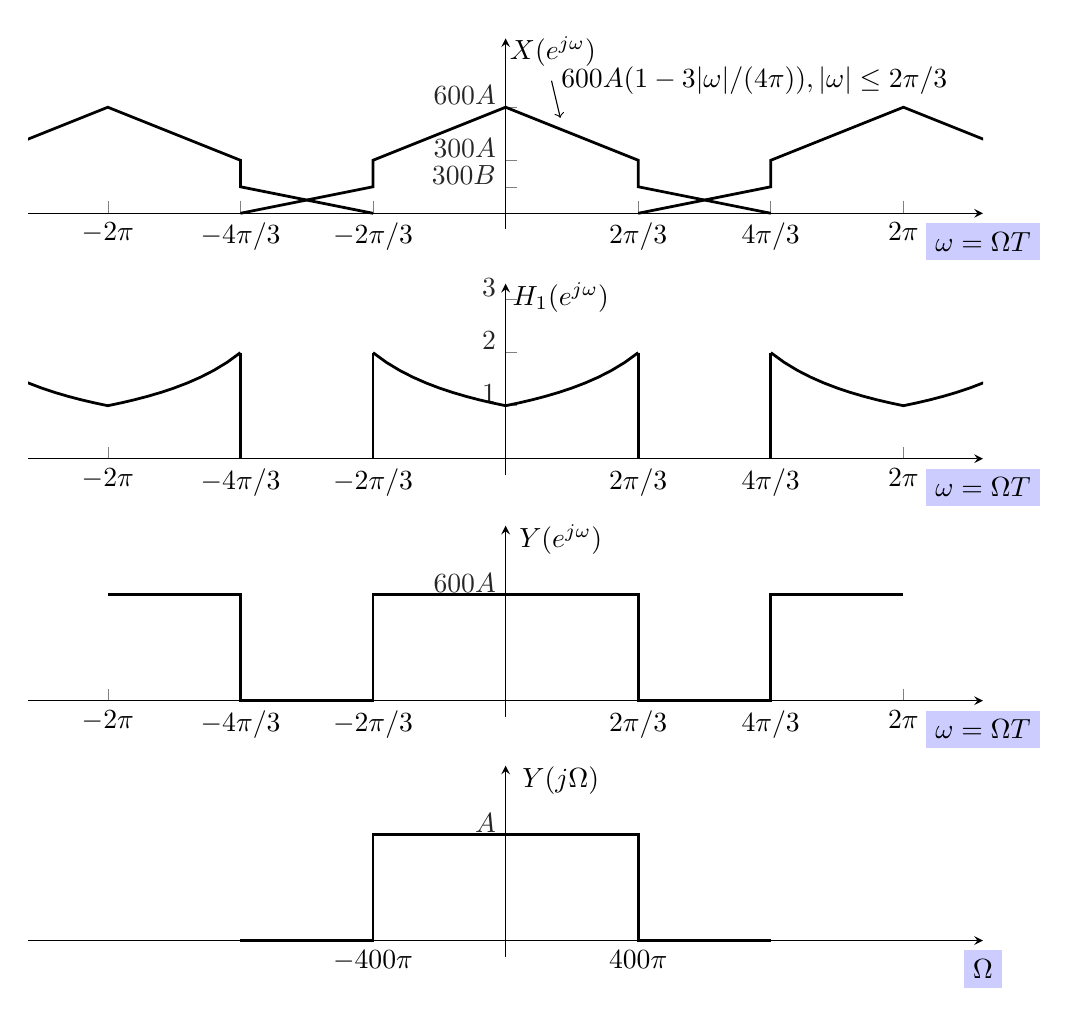
\begin{tikzpicture}
\begin{axis}[
	name=plot1,
	%at=(plot2.below south east), anchor=above north east,
	axis lines*=middle,
	enlargelimits = true,
	clip=true,
	scale only axis,
	width=\textwidth,
	height=0.2\textwidth,
	ymin=0, ymax=3,
	xmin=-8, xmax=8,
	axis line style={->,>=stealth},
	xlabel={\tikz[baseline]{\node[fill=blue!20,anchor=base] (t1) {$\omega = \Omega T$};}},
	ylabel={$X(e^{j\omega})$},
	every axis x label/.style={
		at={(ticklabel* cs:1)},
		%xshift=0.2cm,
		anchor=north,
	},
	every axis y label/.style={
		at={(ticklabel* cs:0.8)},
		anchor=south,
		xshift=0.6cm,
	},
	ytick={0.5, 1, 2},
	yticklabels={$300B$, $300A$, $600A$},
	yticklabel style={yshift=0.15cm},
	xtick={-8, -5.33, -2.666, 2.666, 5.33, 8},
	xticklabels={$-2\pi$, $-4\pi/3$, $-2\pi/3$, $2\pi/3$, $4\pi/3$, $2\pi$}, 
	every outer y axis line/.append style={white!15!black},
	every y tick label/.append style={font=\color{white!15!black}},
	legend style={draw=white!15!black,fill=white,legend cell align=left}]
	\addplot[solid, line width=1pt] coordinates {(-16/3, 0) (-8/3, 1/2) (-8/3, 1) (0, 2) (8/3, 1) (8/3, 1/2) (16/3, 0)};
	\addplot[solid, line width=1pt] coordinates {(-16/3-8, 0) (-8/3-8, 1/2) (-8/3-8, 1) (0-8, 2) (8/3-8, 1) (8/3-8, 1/2) (16/3-8, 0)};
	\addplot[solid, line width=1pt] coordinates {(-16/3+8, 0) (-8/3+8, 1/2) (-8/3+8, 1) (0+8, 2) (8/3+8, 1) (8/3+8, 1/2) (16/3+8, 0)};
	\node (t1) at (axis cs: 5, 2.5) {$600A(1-3|\omega|/(4\pi)), |\omega|\leq2\pi/3$};
	\draw[->] (t1.west) to (axis cs: 1.1, 1.8) {};
\end{axis}

\begin{axis}[
	name=plot2,
	at=(plot1.below south east), anchor=above north east,
	axis lines*=middle,
	enlargelimits = true,
	clip=true,
	scale only axis,
	width=\textwidth,
	height=0.2\textwidth,
	ymin=0, ymax=3,
	xmin=-8, xmax=8,
	axis line style={->,>=stealth},
	xlabel={\tikz[baseline]{\node[fill=blue!20,anchor=base] (t1) {$\omega = \Omega T$};}},
	ylabel={$H_1(e^{j\omega})$},
	every axis x label/.style={
		at={(ticklabel* cs:1)},
		%xshift=0.2cm,
		anchor=north,
	},
	every axis y label/.style={
		at={(ticklabel* cs:0.8)},
		anchor=south,
		xshift=0.7cm,
	},
	yticklabel style={yshift=0.15cm},
	xtick={-8, -5.33, -2.666, 2.666, 5.33, 8},
	xticklabels={$-2\pi$, $-4\pi/3$, $-2\pi/3$, $2\pi/3$, $4\pi/3$, $2\pi$}, 
	every outer y axis line/.append style={white!15!black},
	every y tick label/.append style={font=\color{white!15!black}},
	legend style={draw=white!15!black,fill=white,legend cell align=left}]
	\addplot[solid, line width=1pt, domain=-2.6667:2.6667, samples=21] {(1/(1-3*abs(x*pi/4)/(4*pi)))};
	\addplot[solid, line width=1pt, domain=-2.6667:2.6667, samples=21] ({x-8}, { 1/(1-3*abs(x*pi/4)/(4*pi))});
	\addplot[solid, line width=1pt, domain=-2.6667:2.6667, samples=21] ({x+8}, { 1/(1-3*abs(x*pi/4)/(4*pi))});
	\addplot[solid, line width=1pt] coordinates {(-2.6667, 2) (-2.6667, 0)};
	\addplot[solid, line width=1pt] coordinates {(2.6667, 2) (2.6667, 0)};
	\addplot[solid, line width=1pt] coordinates {(-2.6667+8, 2) (-2.6667+8, 0)};
	\addplot[solid, line width=1pt] coordinates {(2.6667-8, 2) (2.6667-8, 0)};
\end{axis}

\begin{axis}[
name=plot3,
at=(plot2.below south east), anchor=above north east,
axis lines*=middle,
enlargelimits = true,
clip=true,
scale only axis,
width=\textwidth,
height=0.2\textwidth,
ymin=0, ymax=3,
xmin=-8, xmax=8,
axis line style={->,>=stealth},
xlabel={\tikz[baseline]{\node[fill=blue!20,anchor=base] (t1) {$\omega = \Omega T$};}},
ylabel={$Y(e^{j\omega})$},
every axis x label/.style={
	at={(ticklabel* cs:1)},
	%xshift=0.2cm,
	anchor=north,
},
every axis y label/.style={
	at={(ticklabel* cs:0.8)},
	anchor=south,
	xshift=0.7cm,
},
yticklabel style={yshift=0.15cm},
ytick=2,
yticklabels=$600A$,
xtick={-8, -5.33, -2.666, 2.666, 5.33, 8},
xticklabels={$-2\pi$, $-4\pi/3$, $-2\pi/3$, $2\pi/3$, $4\pi/3$, $2\pi$}, 
every outer y axis line/.append style={white!15!black},
every y tick label/.append style={font=\color{white!15!black}},
legend style={draw=white!15!black,fill=white,legend cell align=left}]
\addplot[solid, line width=1pt] coordinates {(-8, 2) (2.6667-8, 2) (2.6667-8, 0) (-2.6667, 0) (-2.6667, 2) (2.6667, 2) (2.6667, 0) (-2.6667+8, 0) (-2.6667+8, 2) (8, 2)};
\end{axis}

\begin{axis}[
name=plot4,
at=(plot3.below south east), anchor=above north east,
axis lines*=middle,
enlargelimits = true,
clip=true,
scale only axis,
width=\textwidth,
height=0.2\textwidth,
ymin=0, ymax=3,
xmin=-8, xmax=8,
axis line style={->,>=stealth},
xlabel={\tikz[baseline]{\node[fill=blue!20,anchor=base] (t1) {$\Omega$};}},
ylabel={$Y(j\Omega)$},
every axis x label/.style={
	at={(ticklabel* cs:1)},
	%xshift=0.2cm,
	anchor=north,
},
every axis y label/.style={
	at={(ticklabel* cs:0.8)},
	anchor=south,
	xshift=0.7cm,
},
yticklabel style={yshift=0.15cm},
ytick=2,
yticklabels=$A$,
xtick={-2.666, 2.666},
xticklabels={$-400\pi$, $400\pi$}, 
every outer y axis line/.append style={white!15!black},
every y tick label/.append style={font=\color{white!15!black}},
legend style={draw=white!15!black,fill=white,legend cell align=left}]
\addplot[solid, line width=1pt] coordinates {(2.6667-8, 0) (-2.6667, 0) (-2.6667, 2) (2.6667, 2) (2.6667, 0) (-2.6667+8, 0)};
\end{axis}
\end{tikzpicture}